




%---------------------------------------------------------------------

\newpage

%\section[Co-evolution at the meso scale][Co-évolution à l'échelle mesoscopique]{Co-evolution of forms: interactions and morphogenesis at the meso scale}{Co-evolution des formes : interactions et morphogenèse à l'échelle mesoscopique}

\section{Co-evolution at the meso scale}{Co-évolution à l'échelle mesoscopique}


\label{sec:mesocoevolmodel}

%---------------------------------------------------------------------


\bpar{
Urban settlements and transportation networks are widely admitted to be co-evolving in the thematic and empirical studies of territorial systems. However, modeling approaches of such dynamical interactions between networks and territories are less developed. We propose to study this issue at an intermediate scale, focusing on morphological and functional properties of the territorial system in a stylized way. We introduce a stochastic dynamical model of urban morphogenesis that couples the evolution of population density within grid cells with a growing road network.
}{
Les établissements urbains et les réseaux de transport ont été montrés comme co-évolutif, dans les différentes approches thématiques, empiriques, et de modélisation des systèmes territoriaux développées jusqu'ici. Comme on l'a vu, les approches modélisant ces interactions dynamiques entre réseaux et territoires sont peu développées. Nous proposons dans cette section de réaliser une première entrée à une échelle intermédiaire, en s'intéressant aux propriétés morphologiques et fonctionnelles des systèmes territoriaux de manière stylisée. Nous introduisons un modèle dynamique et stochastique de morphogenèse urbaine qui couple l'évolution de la densité de population dans les cellules d'une grille avec l'évolution d'un réseau routier.
}


%%%%%%%%%%%%%%%%%%
\subsection{Model}{Description du Modèle}


\subsubsection{Rationale}{Structure générale}


\bpar{
With an overall fixed growth rate, new population aggregate preferentially to a potential for which parameters control the dependance to various explicative variables, namely local density, distance to the network, centrality measures within the network and generalized accessibility. We generalize thus the morphogenesis model studied in~\ref{sec:densitygeneration} with aggregation mechanisms similar to~\cite{raimbault2014hybrid}.
A continuous diffusion of population completes the aggregation to translate repulsion processes generally due to congestion. Because of the different time scales of evolution for urban scape and networks, the network grows at fixed time steps, with rules that can be switched in a multi-modeling fashion. A fixed rule ensure connectivity of newly populated patches to the existing network.
%Two different heuristics are then compared: one based on gravity potential breakdown for which links are created if a generalized interaction potential through a new candidate link exceeds a certain times the potential within the existing network; a second one implementing biological network growth, more precisely a slime mould model.
The different network generation heuristics introduced in~\ref{sec:networkgrowth} are included in the model.
We expect the different heuristics to be complementary since the gravity model would be more typical of planned top-down network evolution, whereas the biological model will translate bottom-up processes of network growth. 
}{
Les principes généraux du modèle sont les suivants. Avec un taux de croissance global fixé, une nouvelle population s'agrège préférentiellement à un potentiel local, dont la dépendance à diverses variables explicatives est contrôlé par des paramètres. Celles-ci sont la densité locale, la distance au réseau, les mesures de centralité dans le réseau et l'accessibilité généralisée. \cite{doi:10.1080/13658816.2014.893347} montre dans le cas de Stockholm la très forte corrélation entre les différents types de centralité et le type d'usage du sol, ce qui confirme l'importance de considérer les centralités comme variables explicatives pour le modèle à cette échelle. Nous généralisons ainsi le modèle de morphogenèse étudié dans~\ref{sec:densitygeneration}, avec des mécanismes d'agrégation similaires à ceux utilisés par~\cite{raimbault2014hybrid}. Une diffusion continue de la population complète l'agrégation pour traduire les processus de répulsion généralement dus à la congestion. A cause des différentes échelles de temps impliquées dans l'évolution de l'environnement urbain et des réseaux, le réseau croit à pas de temps fixes, suivant le sous-modèle développé en~\ref{sec:networkgrowth} : une première règle fixe assure la connectivité des patches nouvellement peuplés au réseau existant. Les différentes heuristiques de génération de réseau sont ensuite incluses dans le modèle. Nous nous attendons à une complémentarité de celles-ci, puisque par exemple le modèle gravitaire sera plus typique d'une évolution de réseau planifiée, tandis que le modèle biologique traduit des processus auto-organisés de croissance de réseau. La Fig.~\ref{fig:mesocoevolmodel:workflow} résume la structure générale du modèle de morphogenèse.
}




%%%%%%%%%%%%%%%
\begin{figure}
	\includegraphics[width=\linewidth]{Figures/MesoCoEvol/mesocoevol}
	\caption[Morphogenesis at the mesoscopic scale][Morphogenèse mesoscopique]{\textbf{Structure of the co-evolution model at the mesoscopic scale.}\label{fig:mesocoevolmodel:workflow}}{\textbf{Structure du modèle de co-évolution à l'échelle mesoscopique.}\label{fig:mesocoevolmodel:workflow}}
\end{figure}
%%%%%%%%%%%%%%%



\subsubsection{Formalization}{Formalisation}


Le modèle est basé sur une grille carrée de population de côté $N$, dont les cellules sont définies par les populations $(P_i)$. Un réseau routier s'y superpose de la même manière qu'en~\ref{sec:networkgrowth}. Nous supposons une distribution de population à l'instant initial ainsi qu'un réseau.


L'évolution des densités se base sur une fonction d'utilité, influencée par des caractéristiques locales de la forme et de la fonction urbaine, que l'on appelle \emph{variable explicative}. Soit $x_k(i)$ une variable explicative locale pour la cellule $i$, qui sera parmi les variables suivantes : 
\begin{itemize}
	\item population $P_i$
	\item distance aux routes
	\item centralité de chemin
	\item centralité de proximité
	\item accessibilité.
\end{itemize}
Pour les trois dernières, celles-ci sont définies comme précédemment pour les noeuds du réseau, puis associées aux cellules en prenant la valeur du noeud le plus proche, pondérée par une fonction décroissante en fonction de la distance à celui-ci\footnote{C'est à dire de la forme $x_k = x^{(n)}_k (\argmin_j d(i,j)) \cdot \exp \left( -  \min_j d(i,j) / d_0 \right)$, avec $x^{(n)}_k$ variable correspondante pour les noeuds, l'indice $j$ étant pris sur l'ensemble des noeuds, et le paramètre de décroissance $d_0$ étant dans notre cas fixé à $d_0 = 1$ pour garder la caractéristique que les variables de réseau sont essentiellement significatives proche de celui-ci.}. Nous considérons alors les variables explicatives normalisées définies par $\tilde{x}_k(i) = x_k(i) - \min_j x_k(j) / (\max_j x_k(j) - \min_j x_k(j))$. 

L'utilité d'une cellule est alors donnée par une agrégation linéaire\footnote{Une alternative étant par exemple une fonction de Cobb-Douglas, qui revient à une agrégation linéaire sur les logarithmes des variables.}
\[
U_i = \sum_k w_k \cdot \tilde{x}_k(i)
\]
où les $\tilde{x}_k$ sont les variables explicatives locales normalisées, et $w_k$ des paramètres de poids, qui permettent de pondérer les différentes influences.


Un pas de temps d'évolution du modèle comporte alors les étapes suivantes :
\begin{enumerate}
	\item Evolution de la population selon des règles similaires au modèle de morphogenèse développé en~\ref{sec:densitygeneration}. Etant donné un taux de croissance exogène $N_G$, les individus sont ajoutés de manière indépendante suivant une agrégation faite selon la probabilité $U_i^\alpha/\sum_k U_k^\alpha$, suivie d'une diffusion aux voisins de force $\beta$, effectuée $n_d$ fois.
	\item Croissance du réseau selon les règles décrites en~\ref{sec:networkgrowth}, sachant que celle-ci a lieu si le pas de temps est un multiple d'un paramètre $t_N$, qui permet d'intégrer un différentiel d'échelles temporelles entre la croissance de la population et celle du réseau.
\end{enumerate}

Les paramètres du modèle que nous ferons varier sont donc :
\begin{itemize}
	\item les paramètres d'agrégation-diffusion $\alpha,\beta,N_g,n_d$, résumés en Table~\ref{tab:density:parameters},
	\item les paramètres de poids des variables explicatives $w_k$, au nombre de 4, compris dans $[0;1]$,
	\item et les paramètres de croissance de réseau des différentes heuristiques, résumés en Table~\ref{tab:networkgrowth:parameters}.
\end{itemize}

Les indicateurs de sortie du modèle sont les indicateurs de morphologie urbaine, les indicateurs topologique du réseau, et les corrélations retardées entre les différentes variables explicatives.


%%%%%%%%%%%%%%%%%%%
\subsection{Results}{Résultats}

\subsubsection{Implementation}{Implémentation}

Le modèle est implémenté en NetLogo, vu l'hétérogénéité des aspects à prendre en compte, et ce langage se montrant particulièrement efficace pour coupler une grille de cellules à un réseau. Les indicateurs de morphologie urbaine sont calculés grâce à une extension NetLogo spécifiquement développée (voir~\ref{app:tools}).


\subsubsection{Experience plan}{Plan d'expérience}

Nous proposons de nous concentrer sur la capacité du modèle à capturer les relations entre réseaux et territoires, et en particulier la co-évolution. Pour cela, nous chercherons si (i) le modèle est capable de reproduire, en plus des indicateurs de forme, les matrices de corrélation statiques calculées en~\ref{sec:staticcorrelations} ; et (ii) le modèle produit une variété de relations dynamiques au sens des régimes de causalité développés en~\ref{sec:causalityregimes}.

Le modèle est initialisé sur configurations entièrement synthétiques, avec une taille de grille $50$. Les configurations sont générées par mélange d'exponentielle : $N_c = 8$ centres sont localisés de manière aléatoire, et une population leur est attribuée selon une loi d'échelle $P_i = P_0\cdot (i+1)^{-\alpha_S}$ avec $\alpha_S = 0.8$ et $P_0 = 200$. La population de chaque centre est distribuée à l'ensemble des cellules avec un noyau exponentiel de forme $d(r) = P_{max}\exp\left( - r / r_0\right)$ où le paramètre $r_0$ est déterminé pour fixer la population à $P_i$, avec $P_max = 20$ (densité au centre)\footnote{On a en effet $P_i = \iint d(r) = \int_{\theta=0}^{2\pi} \int_{r=0}^{\infty} d(r) rdrd\theta = 2 \pi P_{max} \int_r r\cdot \exp\left( - r / r_0\right) = 2 \pi P_{max} r_0^2$, et donc $r_0 = \sqrt{\frac{P_i}{2\pi P_{max}}}$.}. Le squelette de réseau initial est généré comme détaillé en~\ref{sec:networkgrowth}.

Nous explorons un échantillonnage LHS de l'espace des paramètres, avec 10 répétitions pour environ 70,000 points de paramètres, correspondant à un total autour de 700,000 répétitions du modèle\footnote{Pour lesquelles les résultats de simulation sont disponibles également à \url{http://dx.doi.org/10.7910/DVN/OBQ4CS}.}, effectuées sur grille de calcul par l'intermédiaire d'OpenMole.



\subsubsection{Static and Dynamical calibration}{Calibration statique et dynamique}



\bpar{
The model is calibrated at the first order (indicators of urban form and network measures) and at the second order (correlations) with Eurostat population grid coupled with street network from OpenStreetMap through the following workflow: indicators (Moran index, mean distance, hierarchy, entropy for morphology, mean path length, centralities, performance for network) are computed on real areas of width 50km for all Europe (what corresponds to the typical scale of processes the model includes); parameter space of the model is explored using grid computing (with OpenMole model exploration software), from simple synthetic initial configurations (few connected punctual settlements), computing indicators on final simulated configurations; among candidate parameters for given contiguous (in space and indicator space) real areas on which correlations can be computed, the one with the closest correlation matrix computed on repetitions is chosen.
}{
Le modèle est calibré au premier ordre, sur les indicateurs de forme urbaine et de mesure de réseau, ainsi qu'au second ordre sur les correlations entre ceux-ci. Les données réelles utilisées sont toujours celles introduites en~\ref{sec:staticcorrelations}, qui ont le rappelle sont basées sur les données de population raster Eurostat et le réseau routier issu d'OpenStreetMap. Le processus de calibration est le suivant :

}




\bpar{
We obtain a full coverage of real configurations with simulation results in a principal component plan for indicators, for which most of them a close correlation structure is found. Both network heuristics are necessary for the full coverage. The model is thus able to reproduce existing urban form and networks, but also their \emph{interaction} in the sense of correlations.
}{
La Fig.~\ref{fig:mesocoevolmodel:calibration} résume les résultats de la calibration.

}



% insister sur complemetarite des heuirstiques reseau. peu influence celle ci sur morpho urbaine : hypothese : echelles de temps ?
% procedure de calib : iteratif - d'abord indic, puis plus proche matrice de correlation, estimee sur simu proches et repets poru synth, estimee dans l'espace pour reel.

% random heuristic pefform bien sur correlations : correlations nulles. biologique trop contraint dans processus ?



%%%%%%%%%%%%%%%
\begin{figure}
	%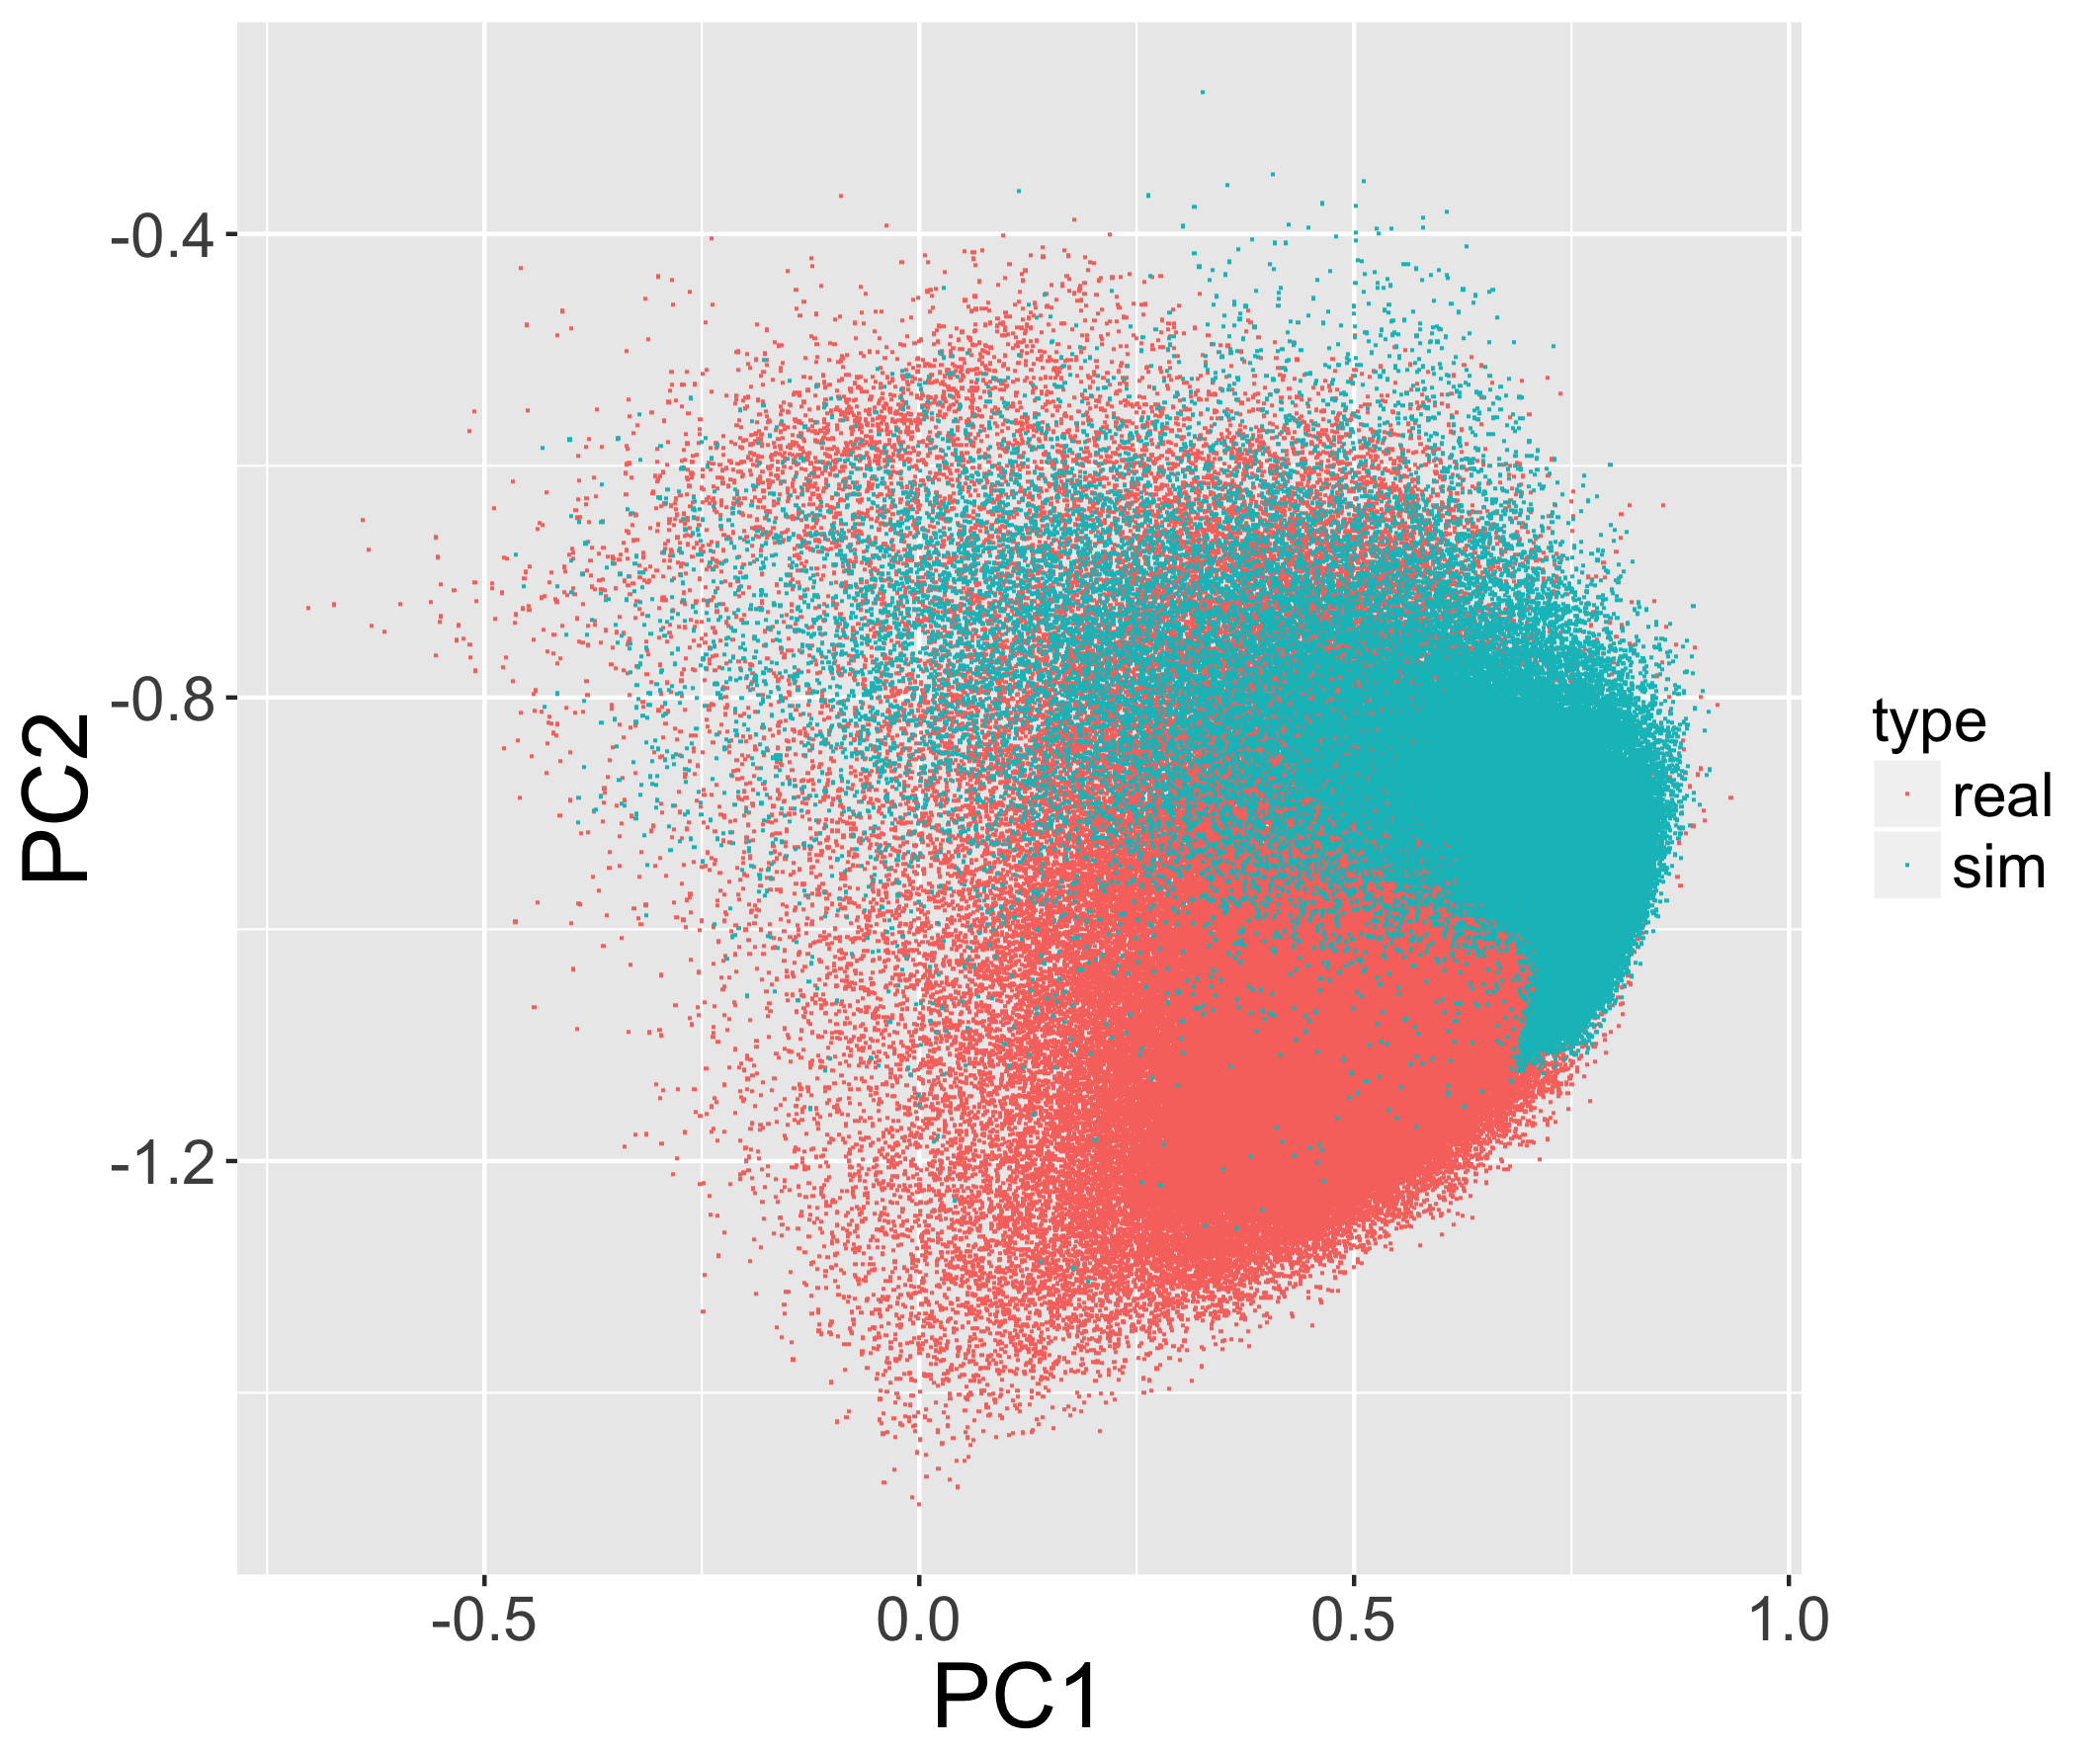
\includegraphics[width=0.48\linewidth]{Figures/MesoCoEvol/pca_allobjs}
	%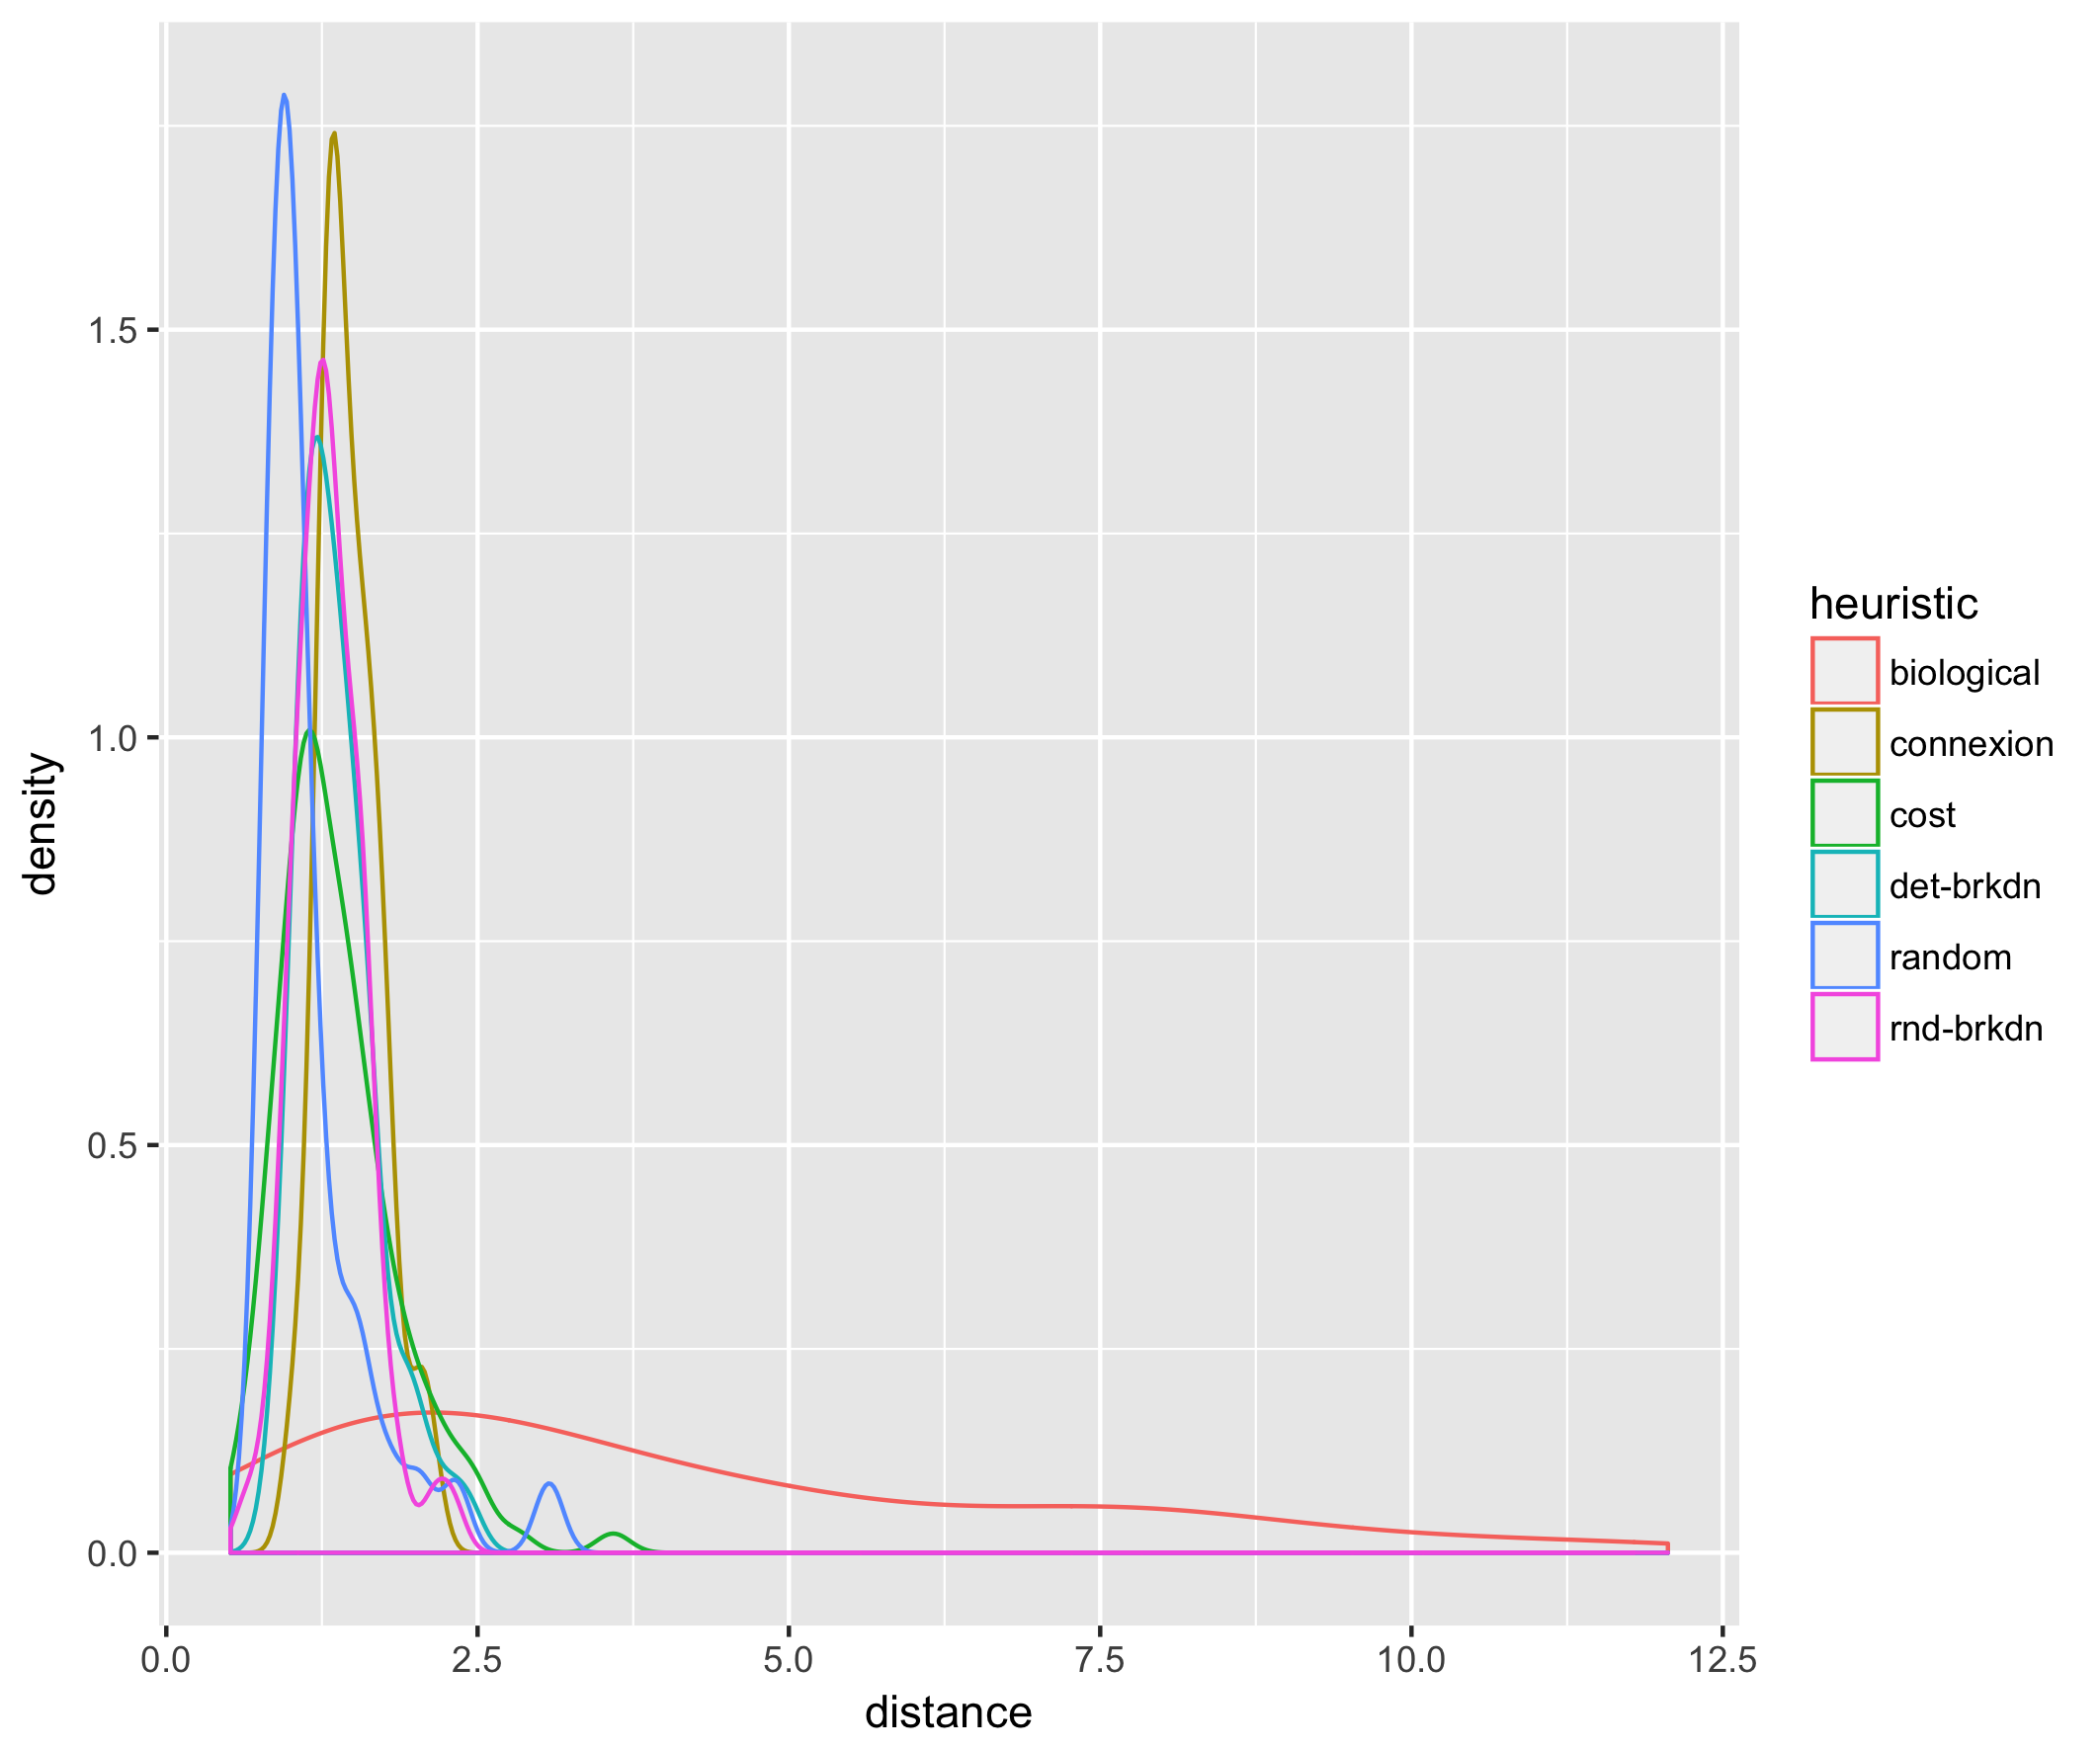
\includegraphics[width=0.48\linewidth]{Figures/MesoCoEvol/corrs-distrib_rhoasize4.png}\\
	%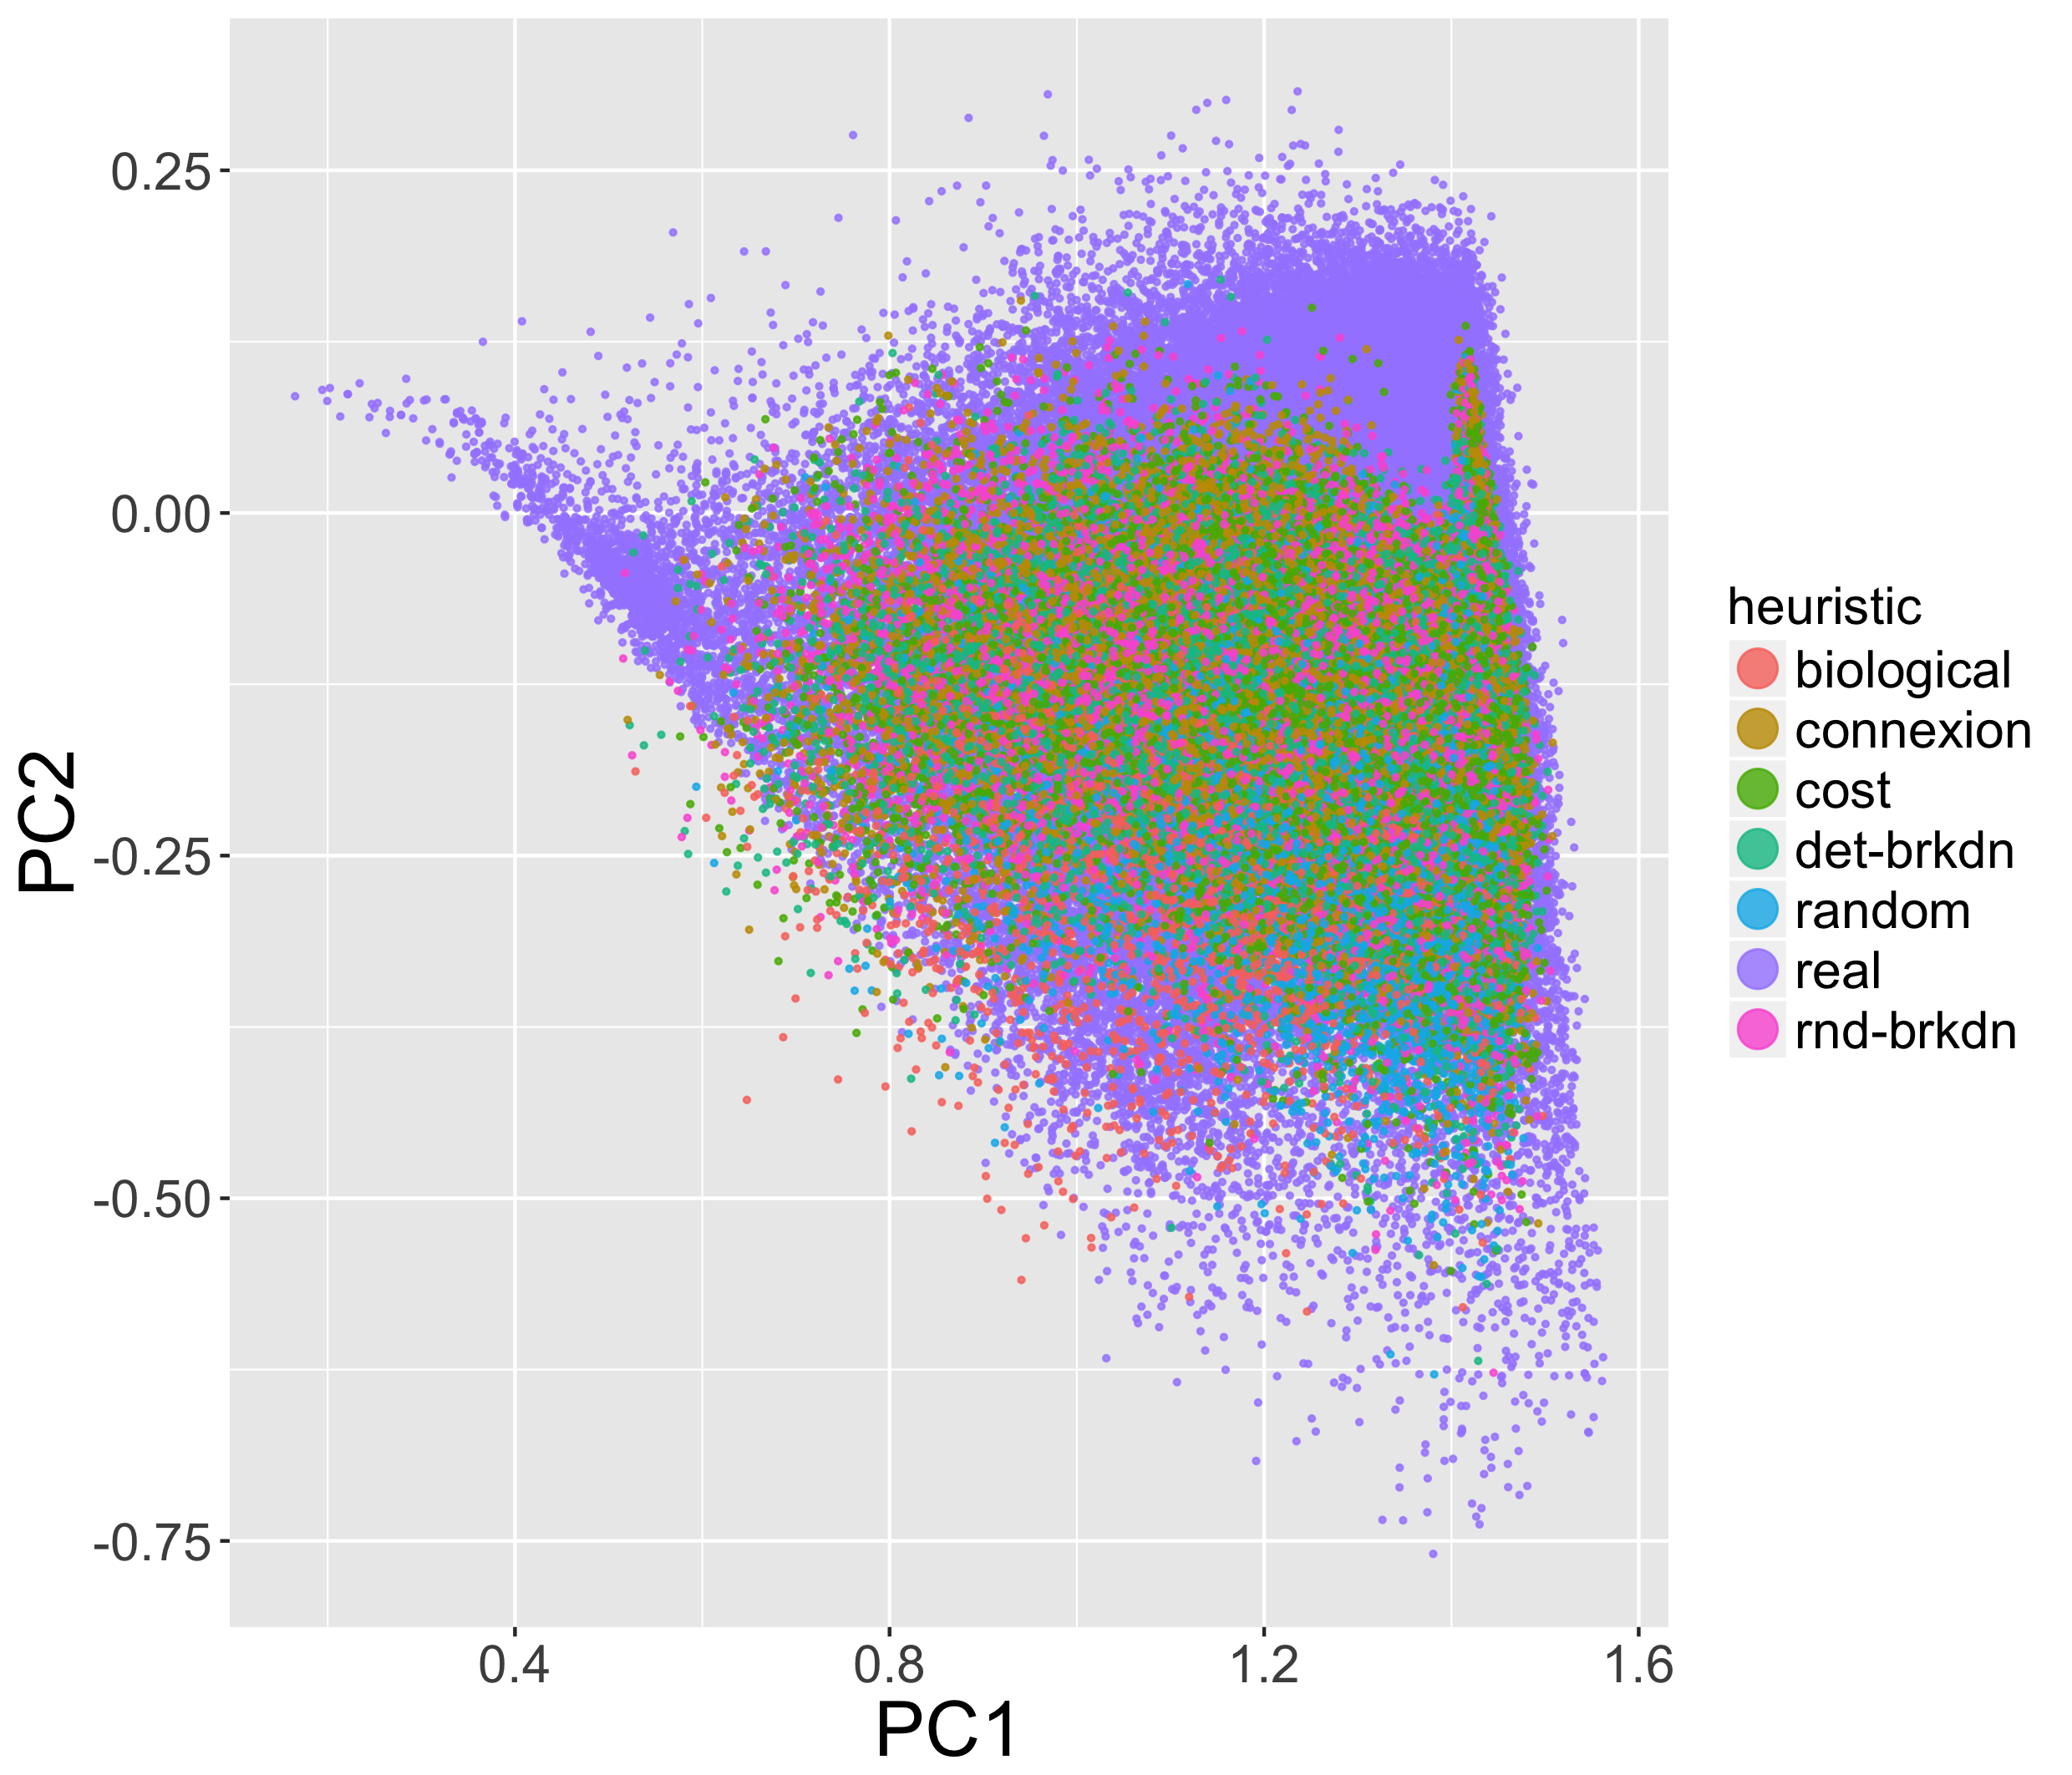
\includegraphics[width=0.48\linewidth]{Figures/MesoCoEvol/pca_morpho_byheuristic}
	%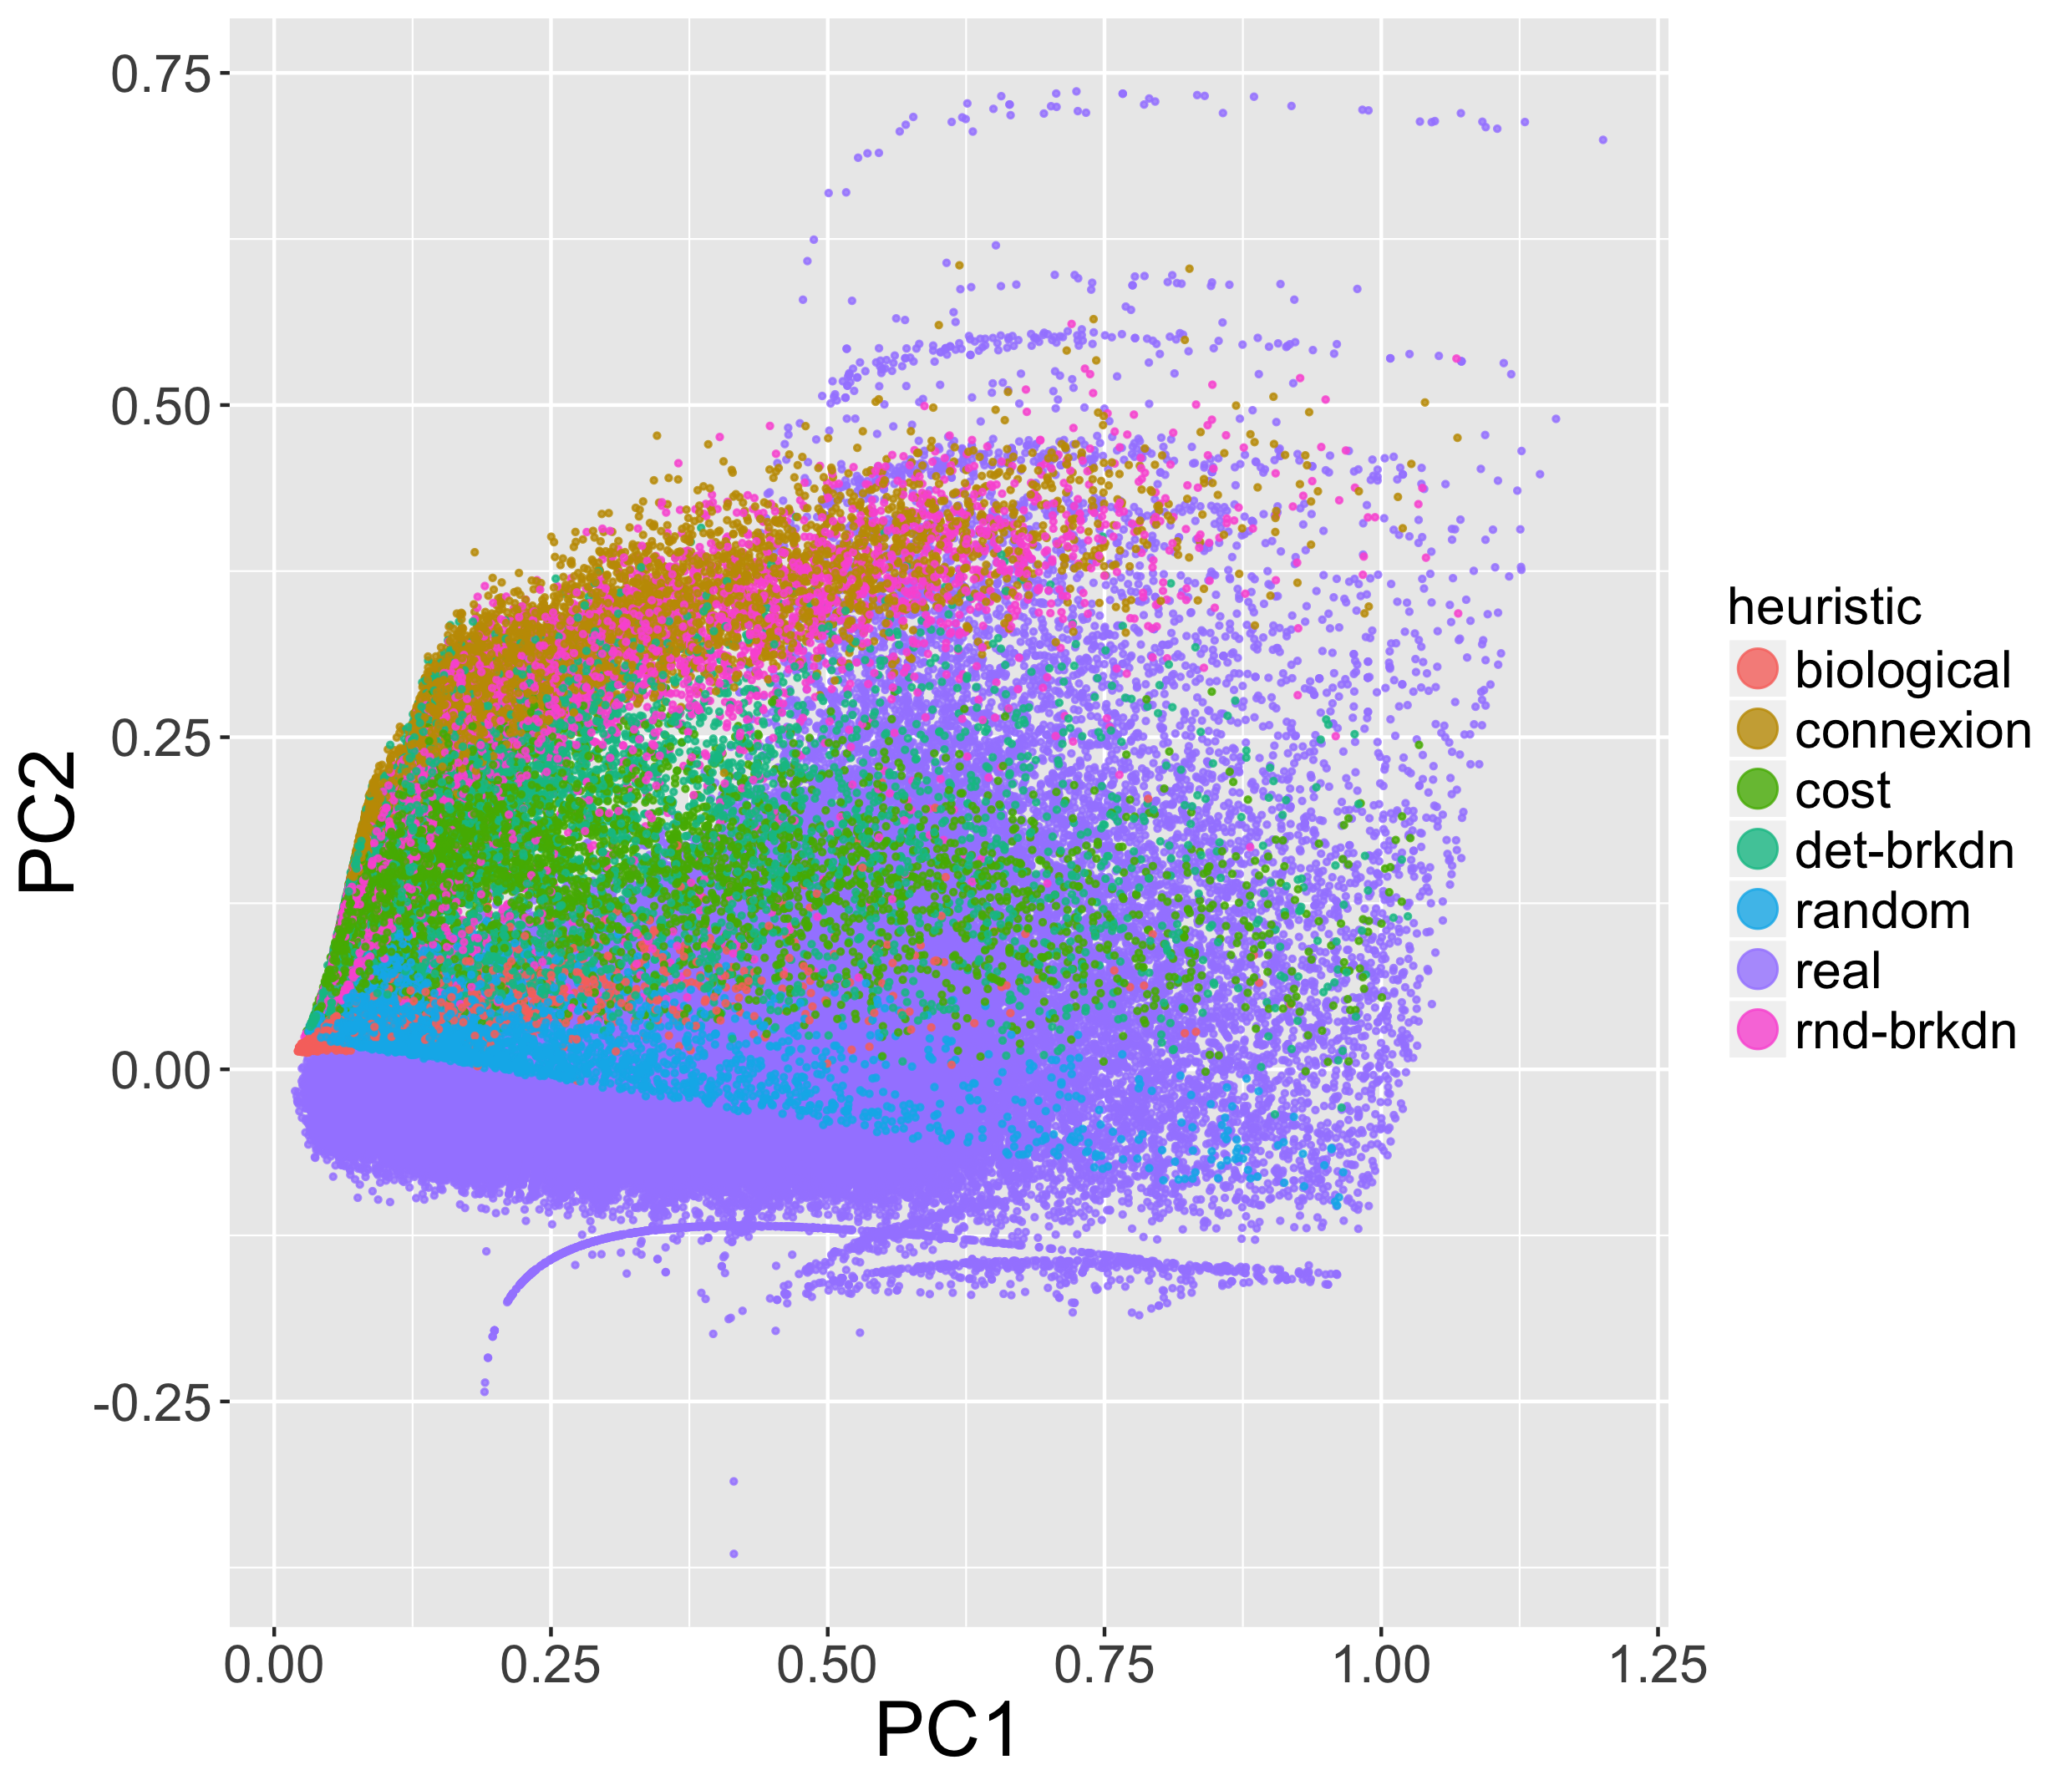
\includegraphics[width=0.48\linewidth]{Figures/MesoCoEvol/pca_network_byheuristic}
	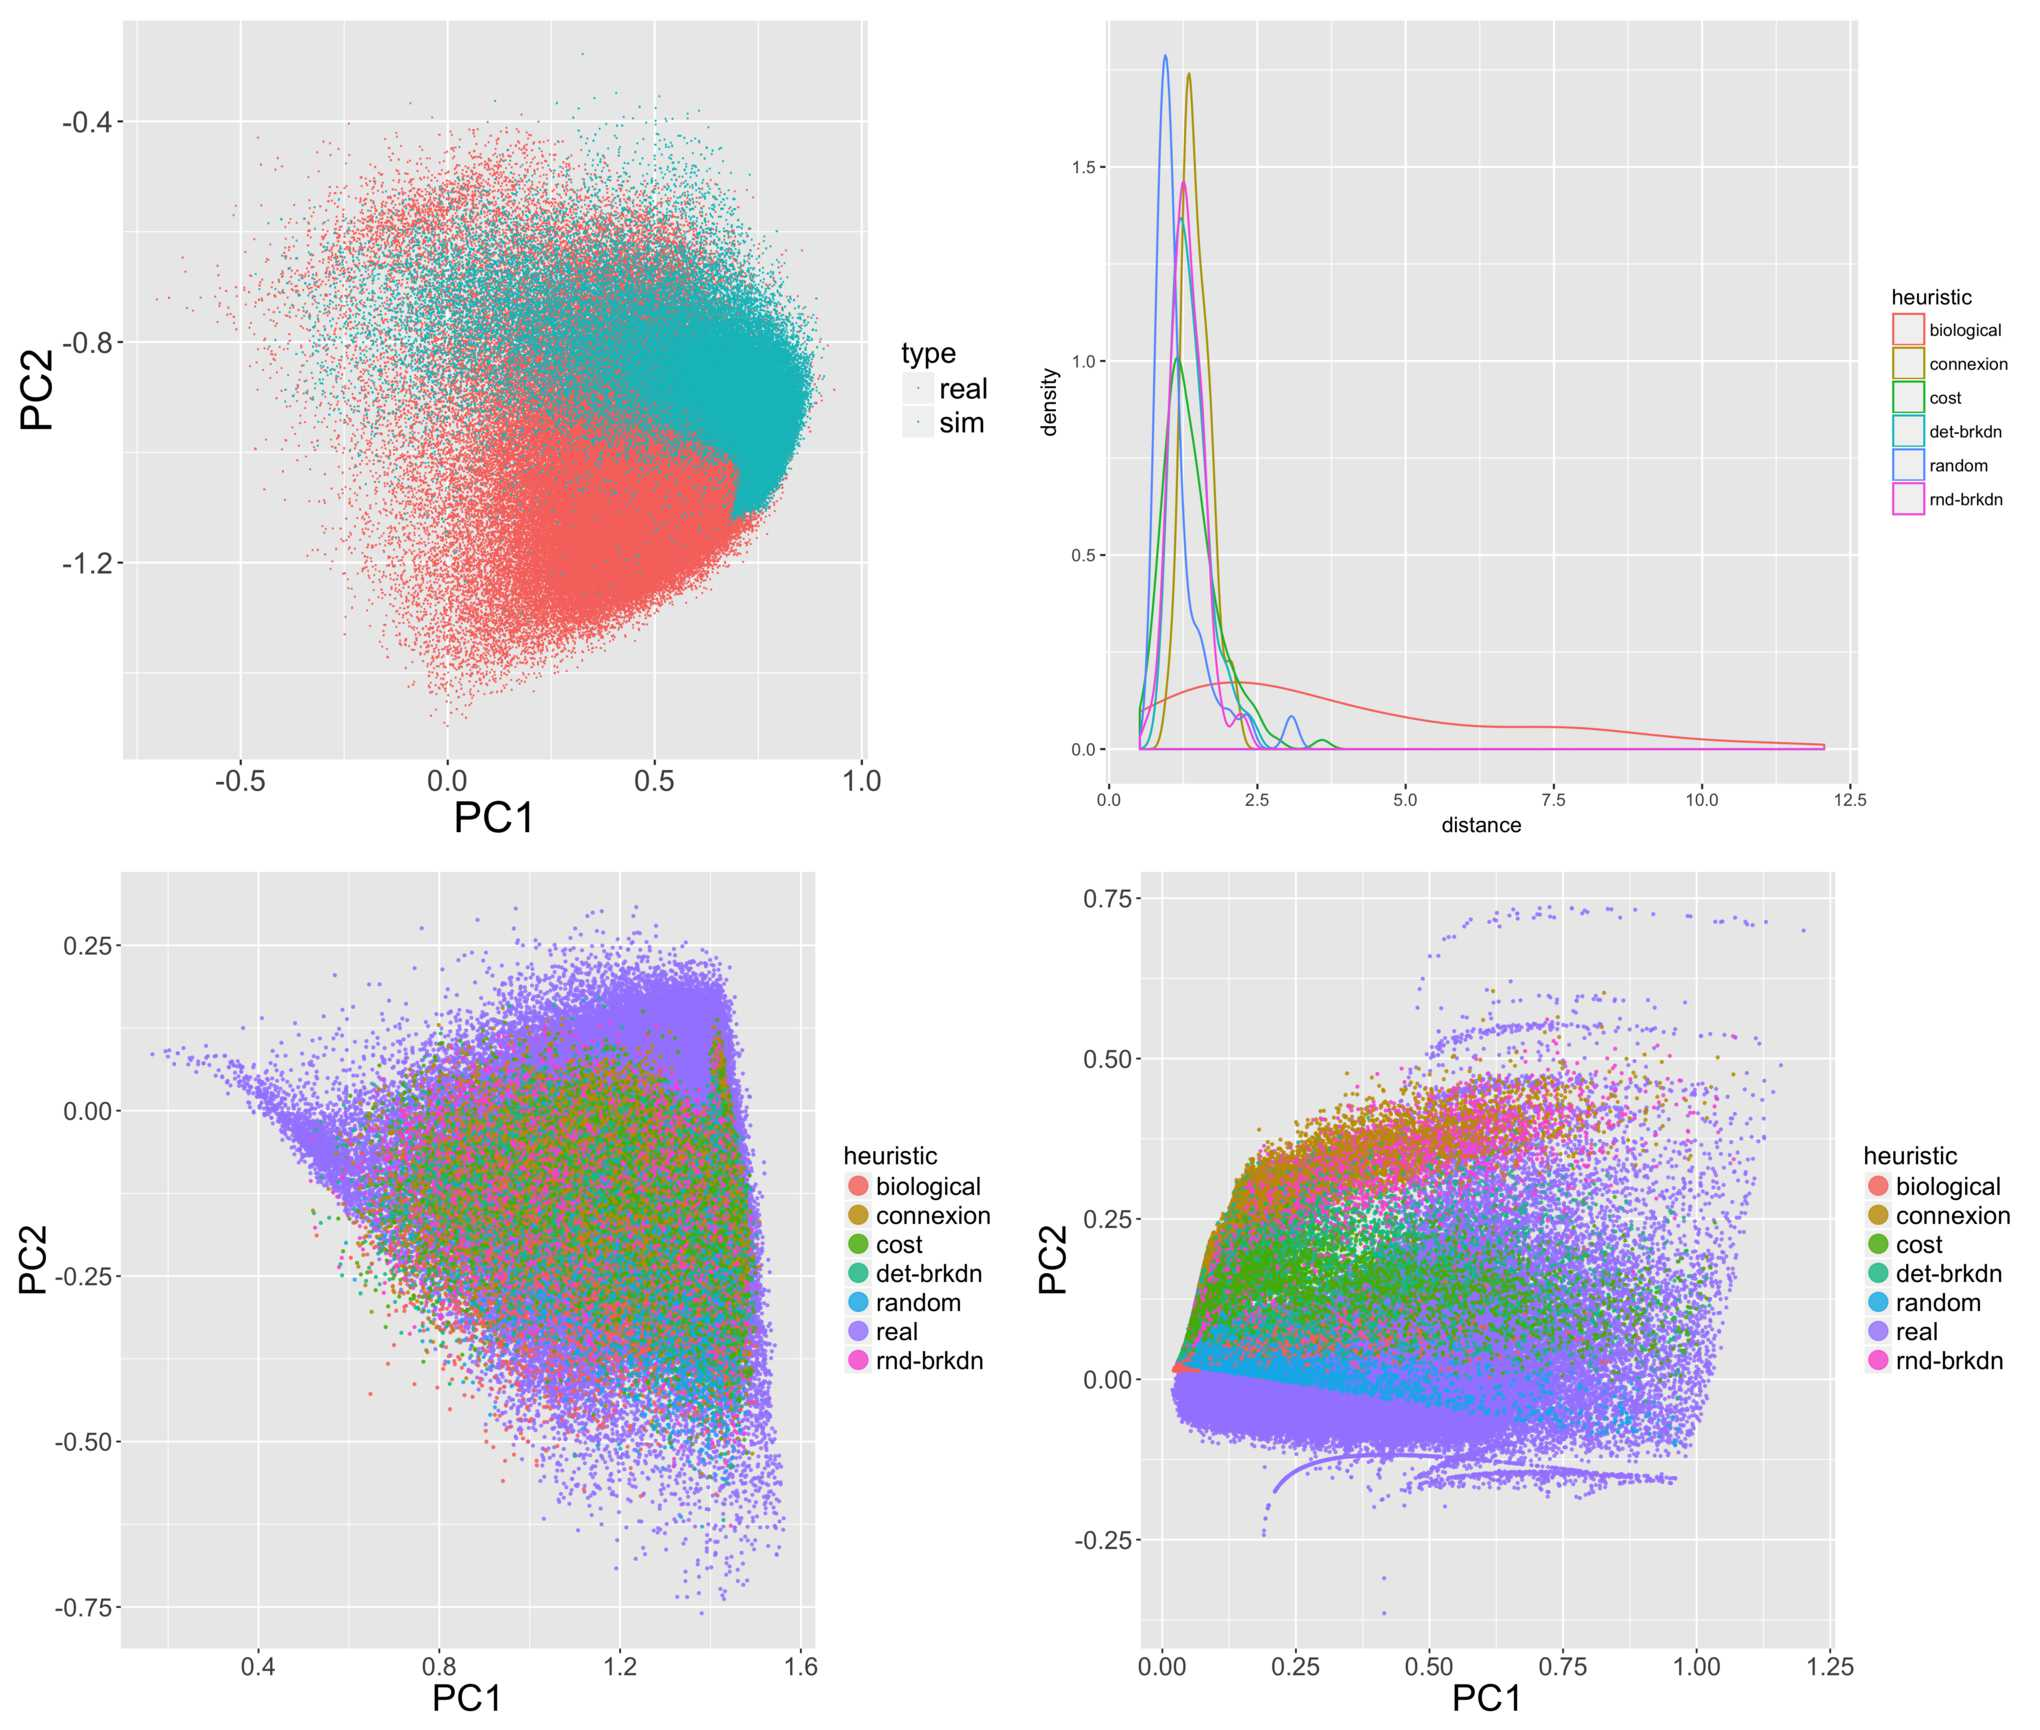
\includegraphics[width=\linewidth]{Figures/Final/7-2-2-fig-mesocoevolmodel-calibration.jpg}
	\caption[Morphogenesis model calibration][Calibration du modèle de morphogenèse]{\label{fig:mesocoevolmodel:calibration}}{\textbf{Calibration du modèle de morphogenèse au premier et au second ordre.} (\textit{Haut Gauche}) Nuages de points simulés et réels dans un plan principal pour l'ensemble des indicateurs. (\textit{Haut Droite})\label{fig:mesocoevolmodel:calibration}}
\end{figure}
%%%%%%%%%%%%%%%





\subsubsection{Causality Regimes}{Régimes de causalité}



\bpar{
We furthermore study dynamical lagged correlations between normalized returns of population and network patch explicatives variables, exhibiting a large diversity of spatio-temporal causality regimes, where network can drive urban growth, the contrary, or more complex circular causalities, suggesting that the model effectively grasps the dynamical richness of interactions.
}{
Nous étudions d'autre part les correlations retardées dynamiques entre les retours normalisés de la population et des variables explicatives des patches, appliquant la méthode des régimes de causalité introduite en~\ref{sec:causalityregimes}. Le modèle exhibe des régimes de causalité divers. Plus précisément, la Fig.~\ref{fig:mesocoevolmodel:causality} résume les résultats obtenus. Le nombre de classe induisant une transition est plus faible que pour le modèle RDB, traduisant un plus faible degré de liberté, et nous fixons dans ce cas $k=4$. Les profils des centroïdes permettent de comprendre la capacité du modèle à capturer plus ou moins une co-évolution.
}

% incluant des causalité circulaires, suggérant qu'il capture effectivement la richesse des interactions dynamiques
% reg 1 : network suit pop ; reg 2 : idem mais pas dans strucutre locale (pop road $\simeq 0$) ; reg3 : nw suit mais que local, pas structure. ; reg 4 : bw anticause access : network and pop avoid congestion ; plus nw suit : somehow circulaire, vraie co-evol ?


%%%%%%%%%%%%%%%
\begin{figure}
	%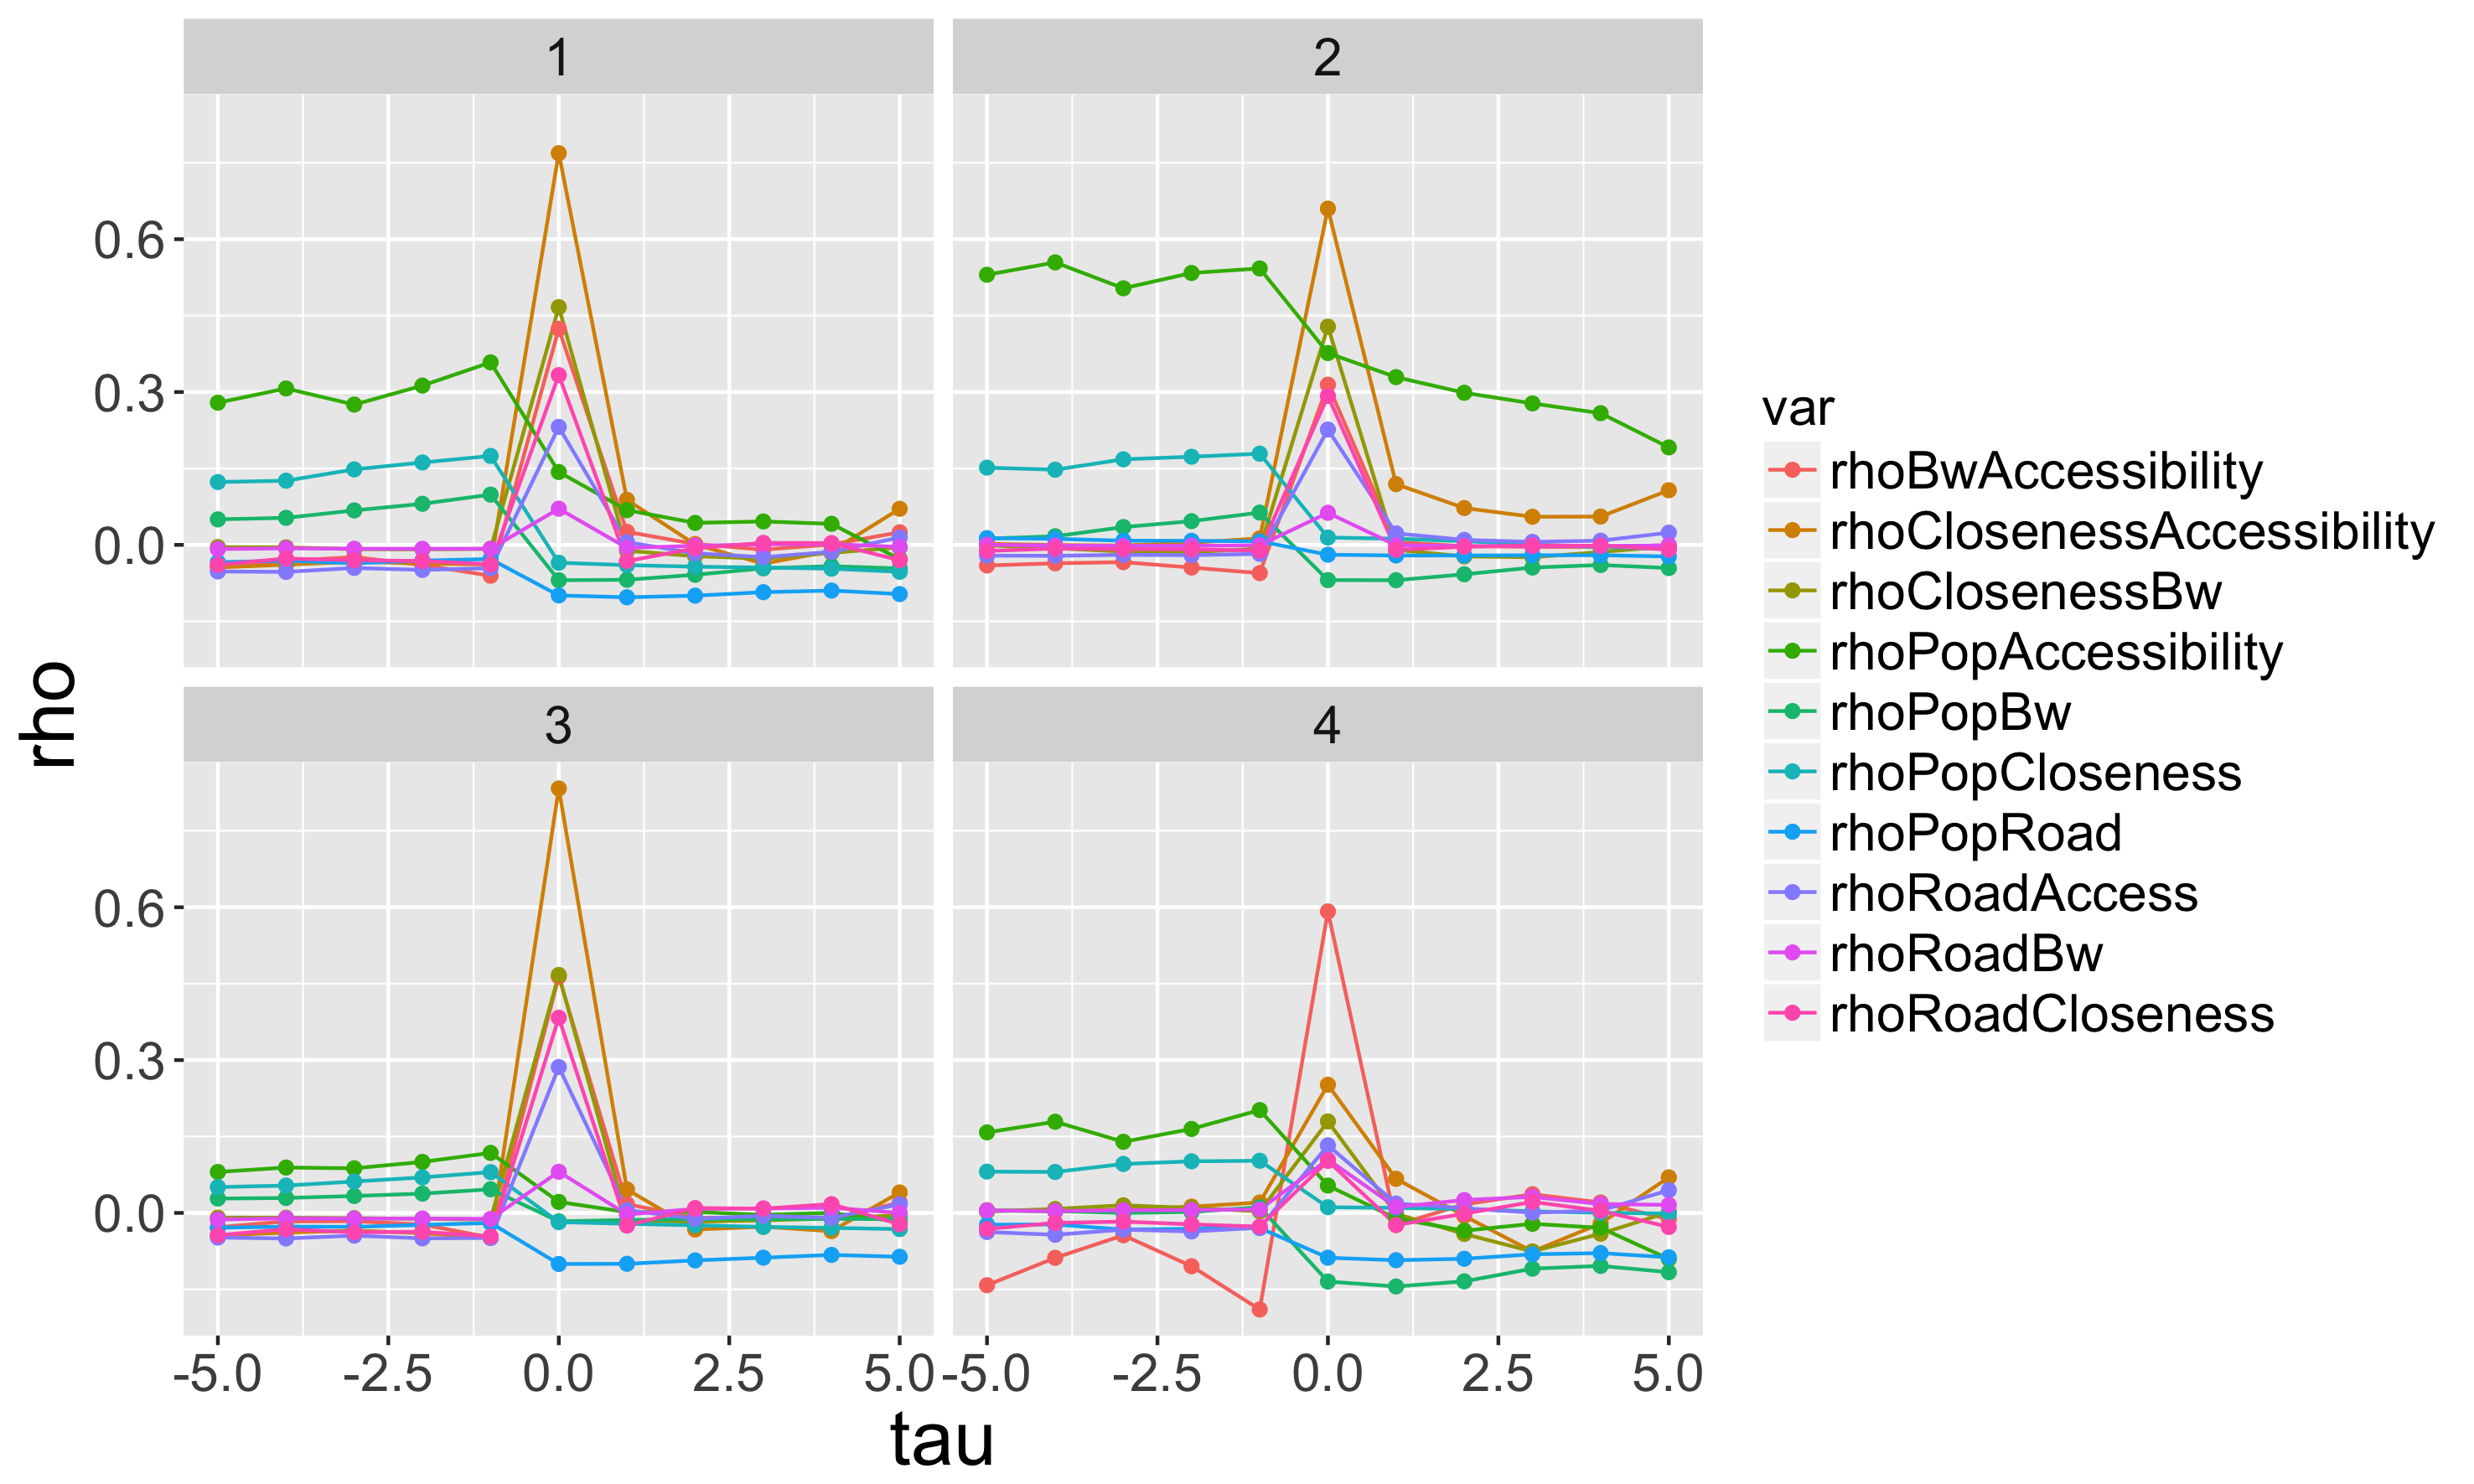
\includegraphics[width=0.53\linewidth]{Figures/MesoCoEvol/centertrajs}
	%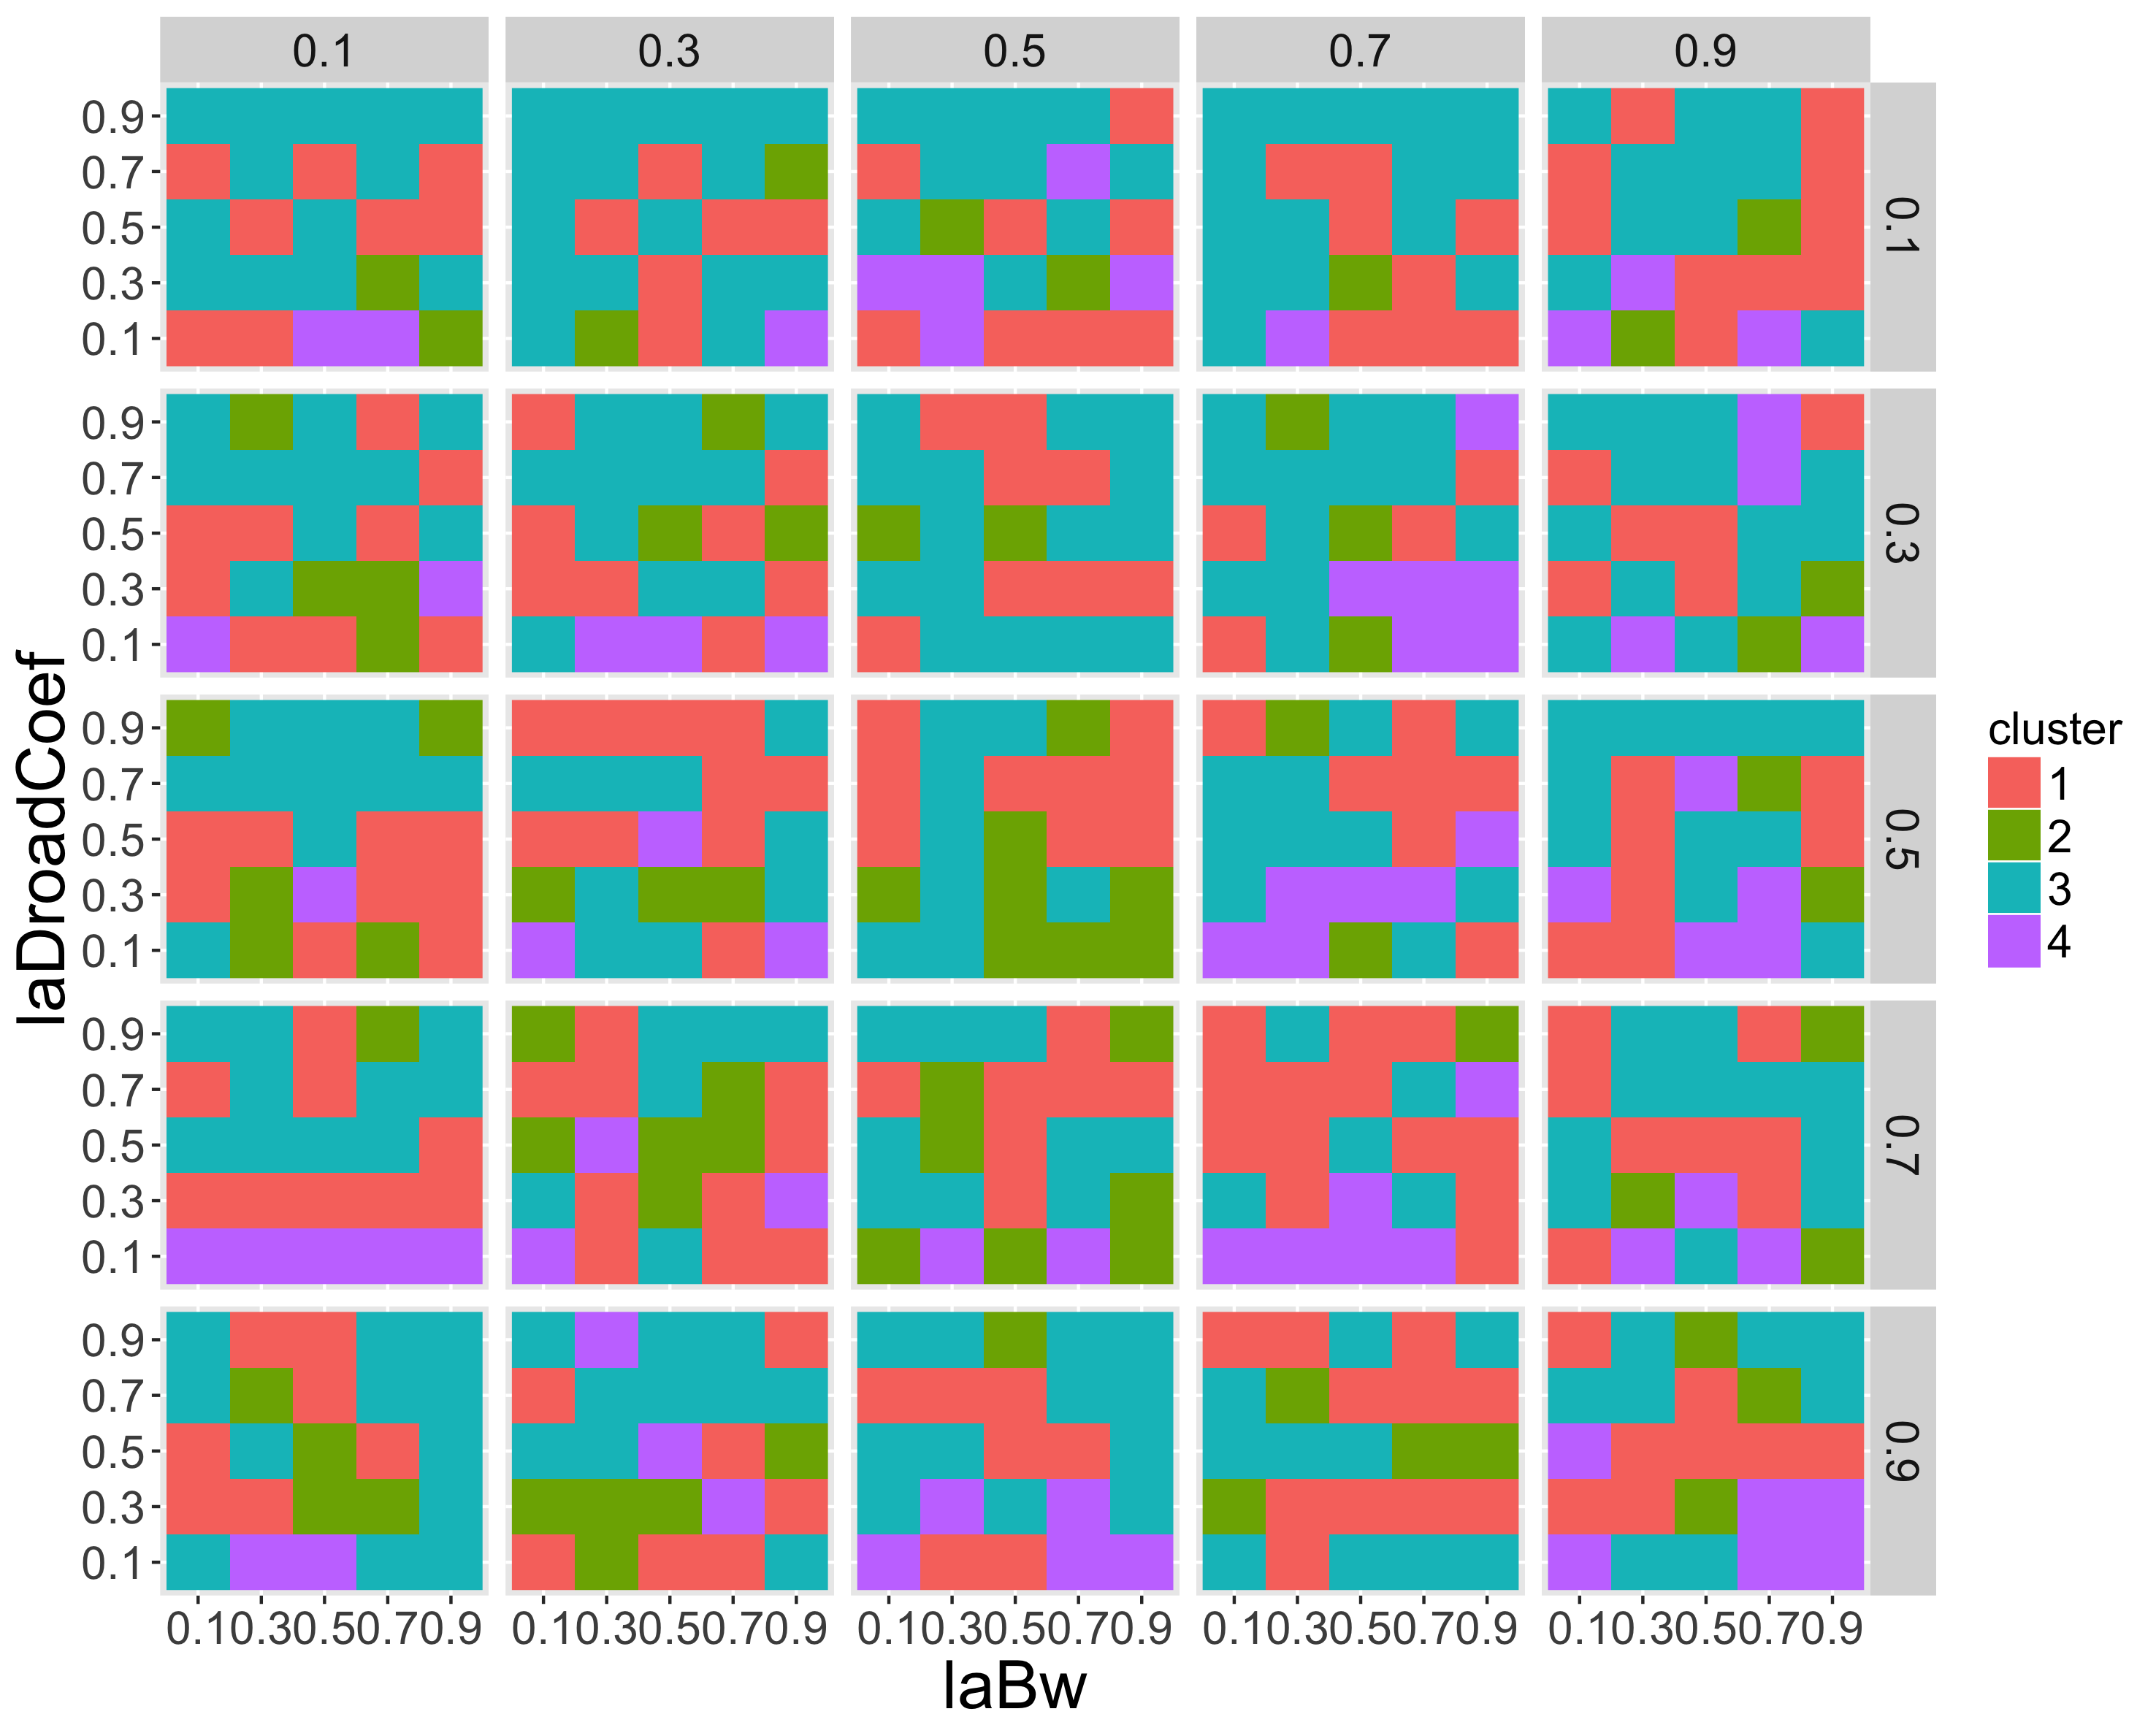
\includegraphics[width=0.44\linewidth]{Figures/MesoCoEvol/cluster-params}
	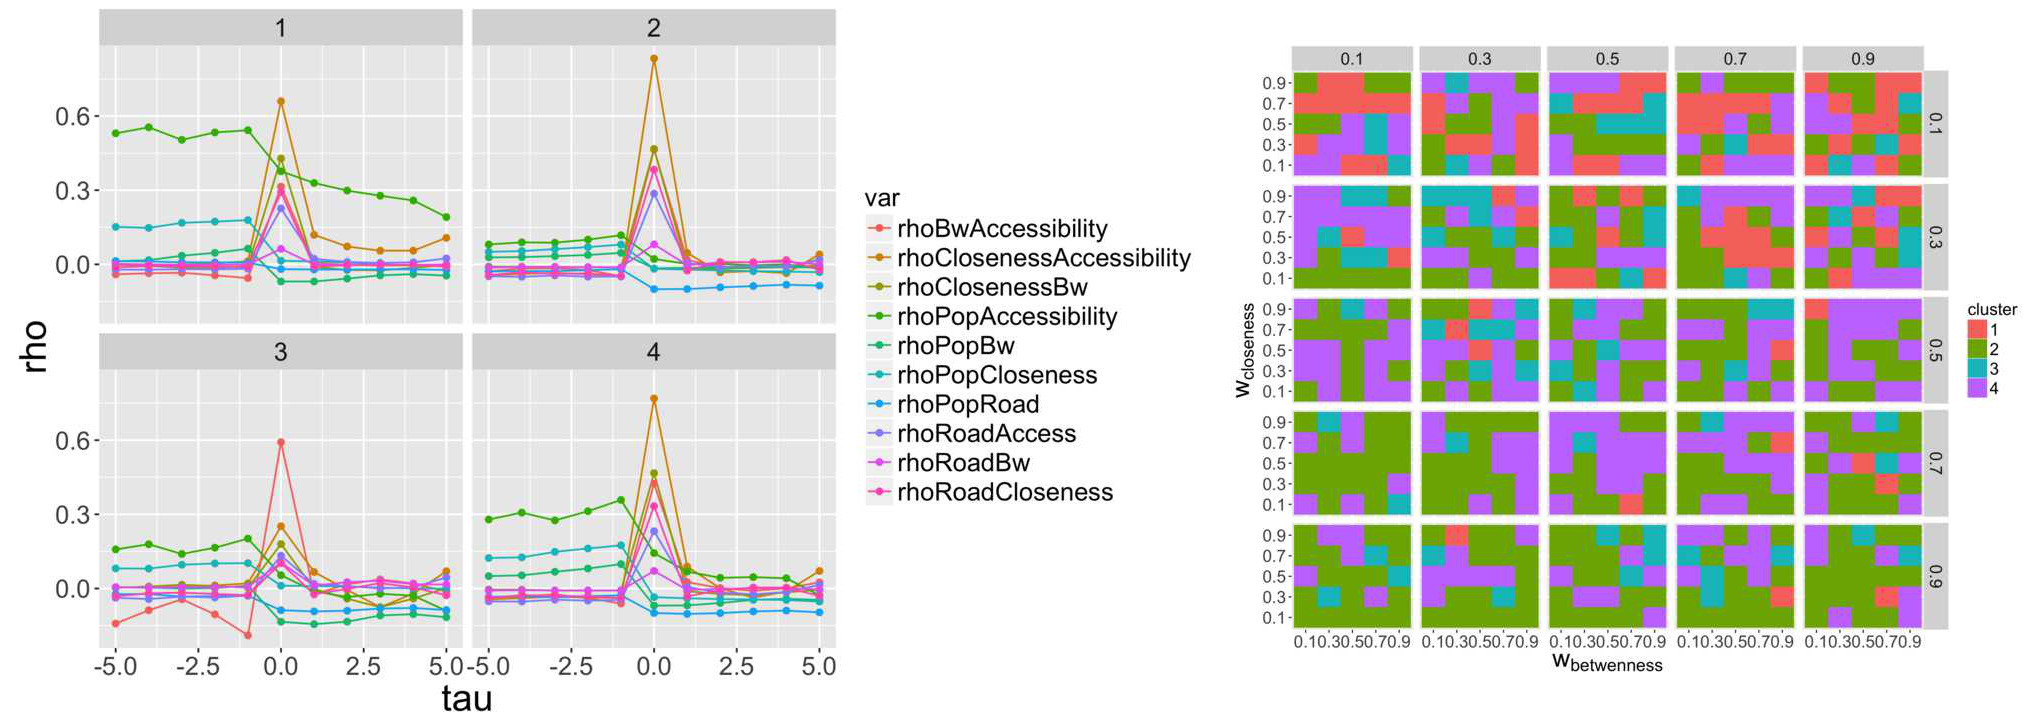
\includegraphics[width=\linewidth]{Figures/Final/7-2-2-fig-mesocoevolmodel-causality}
	\caption[Causality regimes][Régimes de causalité]{}{\textbf{Régimes de causalité.}\label{fig:mesocoevolmodel:causality}}
\end{figure}
%%%%%%%%%%%%%%%





%%%%%%%%%%%%%%%
\subsection{Developments}{Développements}



\comment[JR]{\cite{blumenfeld2010network} : hybrid model (largely discussed by Clara) ; network growth induces migration ; would be interesting to test its abilities to produce various causality regimes (note : may be one indicator of how a model captures co-evolution ?)}


\comment[JR]{develop on Elsa's comment, why just the network with prefatt ? more subtle and want to reproduce coupled dynamics. could suit at the first order ? surely as density-only model performs quite well on morphology only. question of territorial representations, what is necessary, what is an objective, what is both. dimension of urban system.}











